
    \documentclass{standalone}
\usepackage{tkz-fct}
\usepackage{tkz-euclide}
\usepackage{color}
\usepackage{amsmath}
\renewcommand*\familydefault{\sfdefault}
\usepackage{sansmath}
\sansmath
\definecolor{gray75}{gray}{0.75}
\begin{document}
 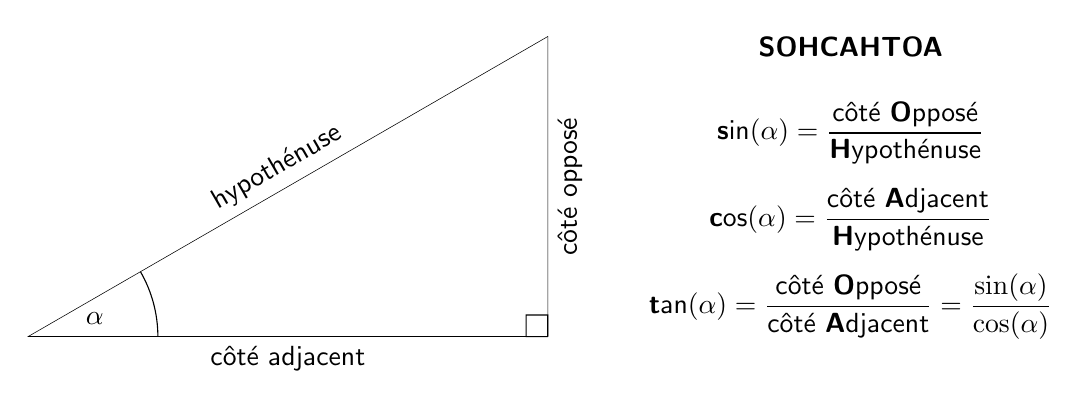
\begin{tikzpicture}[scale=1.1]
   % \tkzInit[xmax=6.0,ymax=6.0,xmin=-6.0 ,ymin=-6.0]
   % \begin{scope}[dashed]
   %   \tkzGrid
   % \end{scope}
   % \tkzDrawX[label={$x$}]
   % \tkzDrawY[label={$y$}]
   % \tkzLabelX
   % \tkzLabelY
\tkzDefPoints{0/0/A,6/0/B}
\tkzDefTriangle[school](A,B)
\tkzGetPoint{C}
\tkzMarkRightAngles(C,B,A)
\tkzLabelSegment[sloped](A,B){côté adjacent}
\tkzLabelSegment[sloped](B,C){côté opposé}
\tkzLabelSegment[above,sloped](A,C){hypothénuse}
\tkzMarkAngle[size=1.5](B,A,C)
\tkzLabelAngle[pos=0.8](B,A,C){$\alpha$}
\tkzDrawSegments(A,B B,C C,A)
\begin{scope}[yshift=-0.65cm,xshift=9.5cm]
\tkzText(0,4){\bf SOHCAHTOA}
\tkzText(0,3){$\text{{\bf s}in}(\alpha)=\dfrac{\text{côté {\bf
        O}pposé}}{\text{{\bf H}ypothénuse}}$}
\tkzText(0,2){$\text{{\bf c}os}(\alpha)=\dfrac{\text{côté {\bf
        A}djacent}}{\text{{\bf H}ypothénuse}}$}
\tkzText(0,1){$\text{{\bf t}an}(\alpha)=\dfrac{\text{côté {\bf
        O}pposé}}{\text{côté {\bf A}djacent}}=\dfrac{\sin(\alpha)}{\cos(\alpha)}$}
\end{scope}

\end{tikzpicture}
\end{document}
